\section{Introduction}
\label{intro}

Diffusion models have emerged as a powerful generative framework, achieving state-of-the-art quality on image synthesis~\cite{Ho20,balaji22,Rombach22,pmlr22,saharia22,Ramesh22}. Recent works harness diffusion models for various image editing and manipulation tasks, including text-guided editing~\cite{Hertz22,Guillaume22,Narek22,avrahami22,Kim22}, inpainting~\cite{Lugmayr22}, and image-to-image translation~\cite{Saharia21,Meng22,Wu22}. A key challenge in these methods is to leverage them for editing of \emph{real} content (as opposed to model-generated images). %\tomer{add more citations in this paragraph.}\inbar{added 4. Saharia21 (Palette) is inpaitning and i2i}% and provide users with control over it.
This requires inverting the generation process, namely extracting a sequence of noise vectors that would reconstruct the given image if used to drive the reverse diffusion process.

Despite significant advancements in diffusion-based editing, inversion is still considered a major challenge, particularly in the denoising diffusion probabilistic model (DDPM) sampling scheme~\cite{Ho20}. Many recent methods (\eg \cite{Hertz22,Mokady22,Narek22,Guillaume22,Bram22,Parmar23}) rely on an approximate inversion method for the denoising diffusion implicit model (DDIM) scheme~\cite{Song21}, which is a deterministic sampling process that maps a single initial noise vector into a generated image. However this DDIM inversion method becomes accurate only when using a large number of diffusion timesteps (\eg 1000), and even in this regime it often leads to sub-optimal results in text-guided editing~\cite{Hertz22,Mokady22}. To battle this effect, some methods fine-tune the diffusion model based on the given image and text prompt~\cite{Bahjat22,Kim22,Valevski22,zhang23}. Other methods intervene in the generative process in various ways, \eg by injecting the attention maps derived from the DDIM inversion process into the text-guided generative process~\cite{Hertz22,Parmar23,Narek22,cao23}.

% , or train a diffusion model to handle specific tasks, such as colorization, inpainting and JPEG restoration~\cite{Saharia21}. \tomer{What about manipulation of attention maps? Regarding image restoration, let's not get into this. There are a ton of papers about this, many of which are not trained for a specific task. Let's only focus on image editing. Add more citations in this paragraph.}\inbar{there is also the automatic mask paper. and SDEdit} 

Here we address the problem of inverting the DDPM scheme. As opposed to DDIM, in DDPM, $T+1$ noise maps are involved in the generation process, each of which has the same dimension as the generated output. Therefore, the total dimension of the noise space is larger than that of the output and there exist infinitely many noise sequences that perfectly reconstruct the image. While this property may provide flexibility in the inversion process, not every consistent inversion (\ie one that leads to perfect reconstruction) is also edit friendly. For example, one property we want from an inversion in the context of text-conditional models, is that fixing the noise maps and changing the text-prompt would lead to an artifact-free image, where the semantics correspond to the new text but the structure remains similar to that of the input image. What consistent inversions satisfy this property? A tempting answer is that the noise maps should be statistically independent and have a standard normal distribution, like in regular sampling. Such an approach was pursued in \cite{Wu22}. However, as we illustrate in Fig.~\ref{fig:generated_vs_us}, this native DDPM noise space is in fact not edit friendly. 

\begin{figure}
% \vskip 0.2in
% \begin{center}
\centering
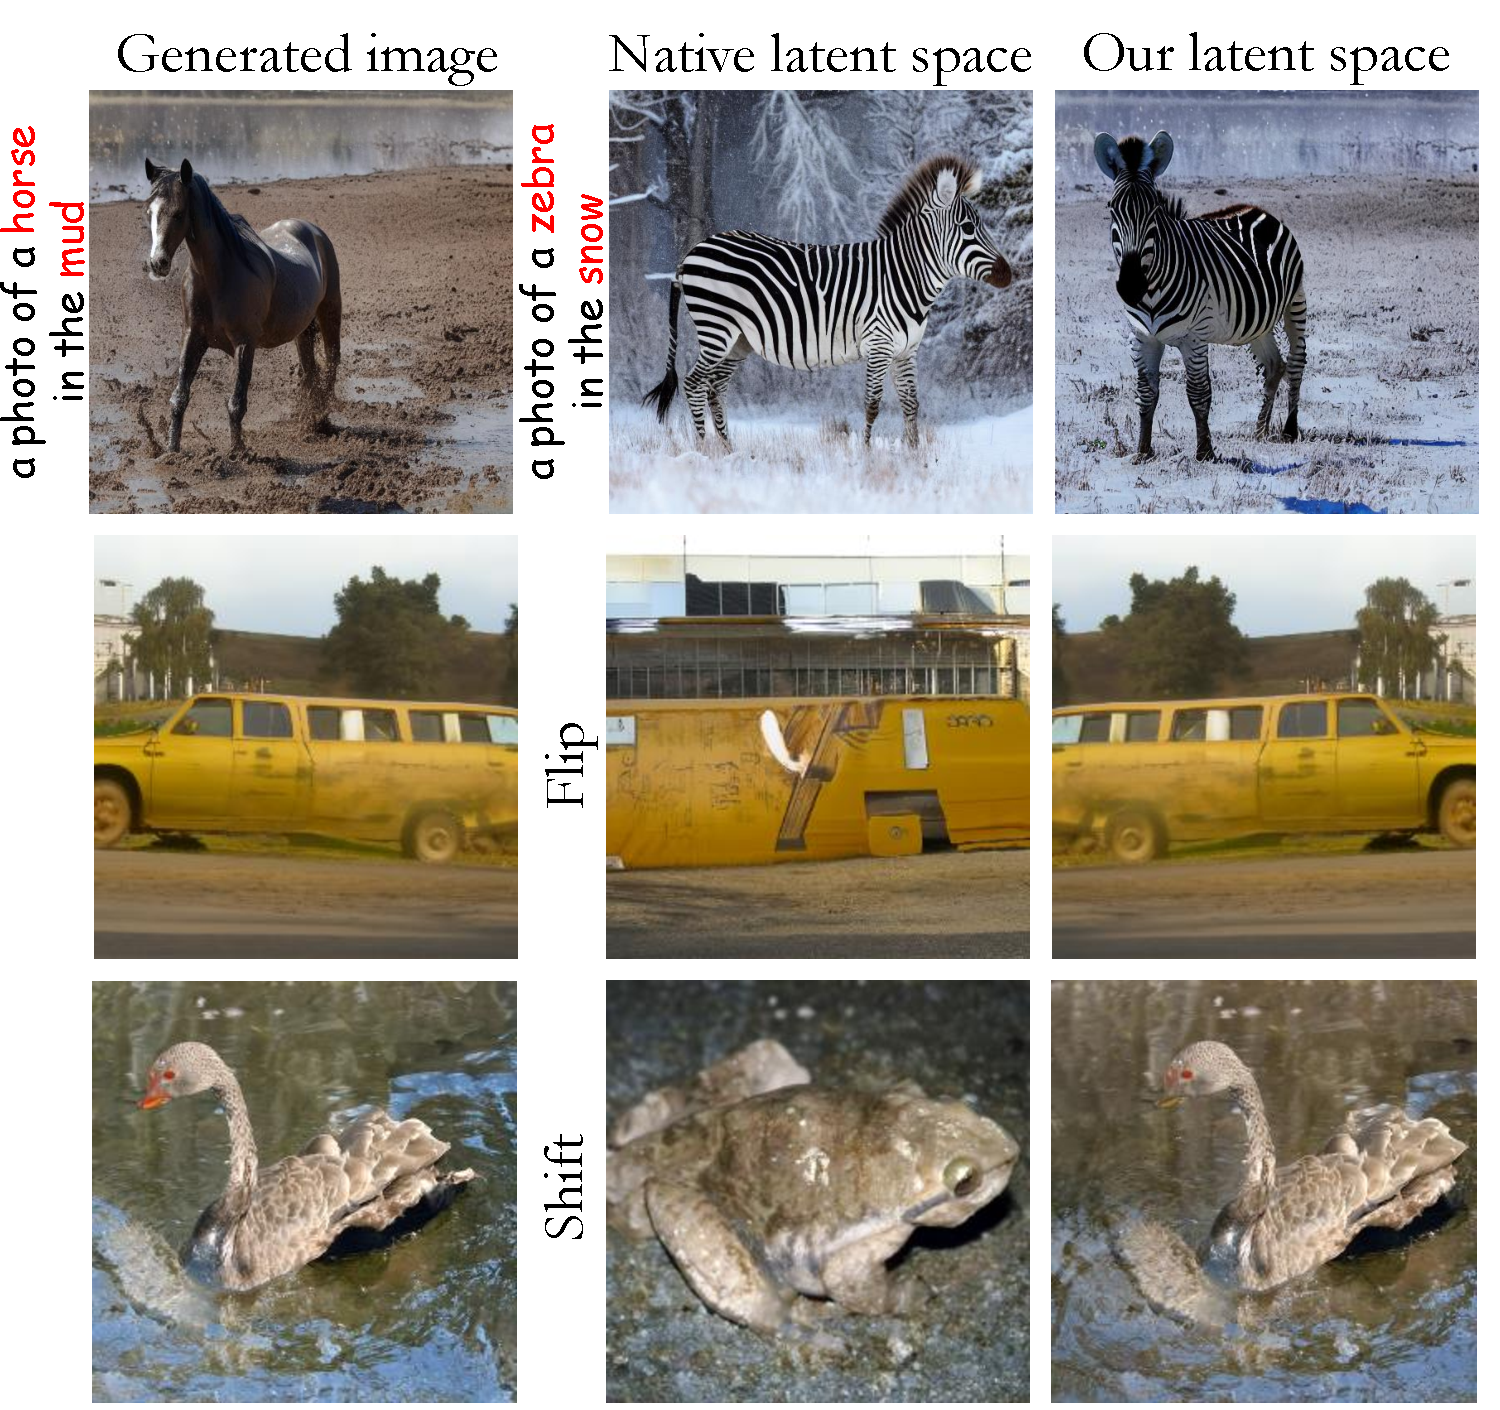
\includegraphics[width=\columnwidth]{ICCV23_submission/figures/generated_vs_us.pdf}
\caption{\textbf{The native and edit friendly noise spaces.} When sampling an image using DDPM (left), there is access to the ``ground truth'' noise maps that generated it. This native noise space, however, is not edit friendly (2nd column). For example, fixing those noise maps and changing the text prompt, changes the image structure (top). Similarly, flipping (middle) or shifting (bottom) the noise maps completely modifies the image. By contrast, our edit friendly noise maps enable editing while preserving structure (right).
}
\label{fig:generated_vs_us}
% \end{center}
% \vskip -0.2in
\end{figure}


Here we present an alternative inversion method, which constitutes a better fit for editing applications, from text-guidance manipulations, to editing via hand-drawn colored strokes. Our inversion ``imprints'' the image more strongly onto the noise maps, which leads to better preservation of structure when fixing them and changing the condition of the model.
% The key idea is to ``imprint'' the image more strongly onto the noise maps, so that they lead to better preservation of structure when fixing them and changing the condition of the model.
% Particularly, our noise maps have higher variances than the native ones, and are strongly correlated across timesteps. 
This is achieved by the fact that our noise maps have higher variances than the native ones. %, and are strongly correlated across timesteps.
Our inversion requires no optimization and is extremely fast. Yet, it allows achieving state-of-the-art results on text-guided editing tasks with a relatively small number of diffusion steps, simply by fixing the noise maps and changing the text condition (\ie without requiring model fine-tuning or intervention in the attention maps). Importantly, our DDPM inversion can also be readily integrated with existing diffusion based editing methods that currently rely on approximate DDIM inversion. As we illustrate in Fig.~\ref{fig:teaser}, this improves their ability to preserve fidelity to the original image. Furthermore, since we find the noise vectors in a stochastic manner, we can provide a diverse set of edited images that all conform to the text prompt, a property not naturally available with DDIM inversion, see top row of Fig.~\ref{fig:teaser} and the Supplementary Supplementary (SM).%fig:variability1,fig:variability2}).





%more image manipulations. Moreover, it can be integrated with existing methods that struggle with real image editing due to their approximation inversion usage. 

%In this paper, we present an inversion process for a pre-trained DDPM that perfectly reconstructs the input image without any training. This inversion can be then used for various editing purposes such as text-editing guidance, hand-drawn colored strokes guidance, and more image manipulations. Moreover, it can be integrated with existing methods that struggle with real image editing due to their approximation inversion usage.
 
%Given an image, we extract the initial and the intermediate noise vectors that reconstruct the image in the generative process. These extracted vectors show high variance and correlation with each other, contrary to the noise vector used to generate a fake image. While Wu et al~\cite{Wu22} suggested a DDPM-inversion that recovers uncorrelated noise vectors from Gaussian distribution, they do not show editing capabilities when using them with different conditions. Figure~\ref{fig:teaser} shows examples for editing with our and Wu et al~\cite{Wu22} extracted noise vectors, as well as with original noise vectors in the case of fake images.

% The key factor is that even if we have the noise vectors, as we have in fake images, or have a good inversion as~\cite{Wu22}, they are not editable, as shown Figure~\ref{fig:teaser}. 

% These properties are opposed to the original noise vectors that are sampled in the generative process.

% The key factor is that even if we have the noise vectors, as we have in fake images, or have a good inversion as~\cite{Wu22}, they are not editable, as shown Figure~\ref{fig:teaser}.

% Since our method inverts the sampling process, it can be applied in pixel space or in the feature space~\cite{Rombach22}.

% Our edited images are faithful to the condition as well as preserve the structure of the input image.




% such as shifting them, interpolate them with another noise vectors or changing them using a mask with hand-drawn colored strokes, and results in a real image in preserving well the input image content while 
% More specifically, we consider an off-the-shelf pretrained DDPM model and reinterpreting it as a model with $T+1$ inputs, i.e., the starting noise vector $X_T$ and set of the $T$ intermediate noise vectors $z_t$. For a given real image, our method extract these set of inputs. Using these inputs with the sampling process, generated the original real image. However, using them with a different conditioning, generates the structure of the real image with the new conditioning.

% latent space~\cite{Rombach22}. 
% More specifically, the original sampling method of the diffusion models starts with a completely Gaussian noise image $X_T$, and by $T$ steps that each of them denoises part of the noise, it produces a clean real image, $X_0$. The commonly used image synthesis is the stochastic process Denoising Diffusion Probabilistic Models (DDPMs)~\cite{Ho20}. A deterministic generative process is the Denoising Diffusion Implicit Models (DDIMs)~\cite{Song21} which introduce a non-markovian diffusion processes. Both generative processes can also be 


% Rombach et al.~\cite{Rombach22} suggest a latent Diffusion model (LDM) by applying this process over the latent space with a decoder part on top of the denoising process.

% Song et al.~\cite{Song21} suggested a non-Markovian process that results in a deterministic denoising process. 

% However,  balancing faithfulness to the user guidance (e.g., hand-drawn colored strokes or prompt) and realism of the synthesized image is a hard task due to the stochastic nature of the DDPM. 

% \begin{figure}
% \label{fig:reconstruction}
% \vskip 0.2in
% % \begin{center}
% \includegraphics[width=\columnwidth]{figuers/reconstruction.png}
% \caption{Reconstruction quality. All methods use a denoiser model trained with 1000 timesteps. In this comparison, the sampling process is for 50 timesteps.}
% \label{fig:unfold}
% % \end{center}
% % \vskip -0.2in
% \end{figure}

% Since this generative model showed its ability to generate high-resolution detailed images, the research on editing images kept growing
% In order to train this model, real images are transformed into their noisy version, and the model estimates the noise added at a certain timestep. All the above can also be done over the latent space, where the diffusion model is wrapped with an encoder and a decode.
%\inbar{citation from arxiv - are they correct?}
%\inbar{can add asyrp to clip guided diffusion example}
%\inbar{add that a lot of papers keep the structure via attentions, we dont}